\documentclass[10pt,a4paper]{article}
\usepackage[utf8]{inputenc}
\usepackage{amsmath}
\usepackage{gensymb}
\usepackage{amsfonts}
\usepackage{siunitx}
\usepackage[european]{circuitikz}
\usepackage{geometry}
\newgeometry{tmargin=2cm, bmargin=2cm, lmargin=2cm, rmargin=2cm}
\usepackage{amssymb}
\usepackage{multirow}
\usepackage{polski}
\usepackage{graphicx}
\author{\textbf{T. Fąs}}
\title{\textbf{UKŁADY SCALONE}}
\begin{document}
\maketitle

\begin{center}
\textbf{\subsection*{STRESZCZENIE}}
\end{center}
W doświadczeniu badano własności bramek logicznych i układów scalonych oraz zaprojektowano i skonstruowano stoper z opcjami start, stop i reset odliczający od 0 do 99. 


\begin{center}
\textbf{\subsection*{WSTĘP}}
\end{center}

Bramki logiczne to układy elektroniczne zdolne do wykonywania operacji logicznych, takich jak iloczyn, suma czy negacja. Odpowiednikiem "1" jest napięcie 5V, a odpowiednikiem "0" jest brak napięcia na wejściu/wyjściu bramki. Symbole przykładowych bramek logicznych wraz z tabelkami prawdy przedstawiona na Rysunku 1.

\begin{figure}[h!]
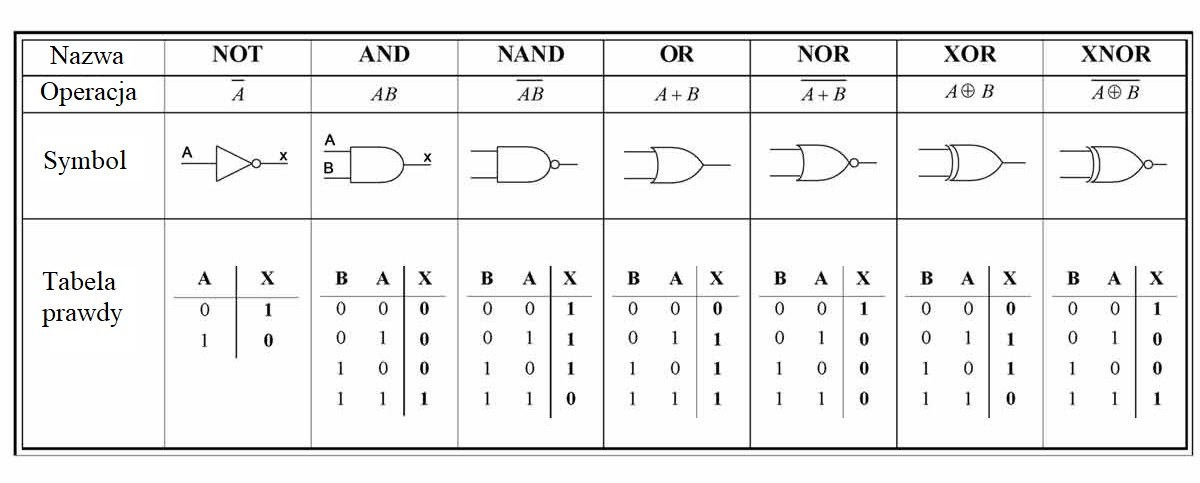
\includegraphics[width=13cm]{rap22rys1} 
\centering
\caption{Przykłady bramek logicznych.}
\end{figure}

Z bramek logicznych można budować układy zdolne do przechowywania wartości logicznych. przykładem takiego układu jest przerzutnik typu D, którego budowę i symbol przedstawiono na Rysunku 2. Tabelka prawdy jest przedstawiona w Tabeli 1.

\begin{figure}[h!]
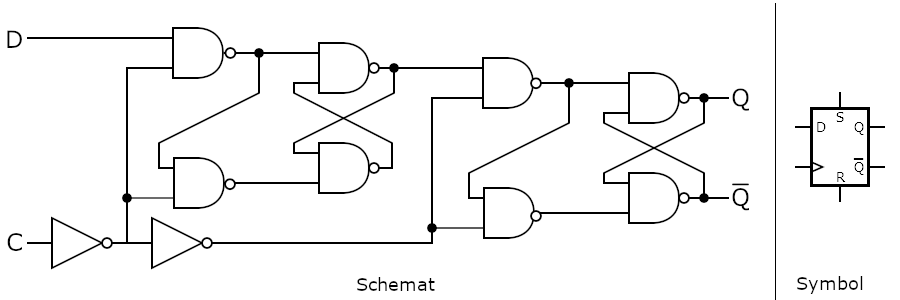
\includegraphics[width=13cm]{rap22rys2} 
\centering
\caption{Przerzutnik typu D.}
\end{figure}


 Przerzutnik typu D reaguje na wzrastające zbocze sygnału zegara C (ozn: trójkąt). Jeśli taki sygnał nie nastąpi, to stan przełącznika się nie zmieni tj. wejście danych D może przyjąć dowolny stan X, a wyjście Q nie zmieni swojego stanu. 

\begin{table}[h!]
\centering
\caption{Tabel prawdy: przerzutnik typu D.}
\begin{tabular}{|c|c|c|}
\hline
Zegar   & D & Q \\ \hline
Wzrasta & 0 & 1 \\ \hline
Wzrasta & 1 & 1 \\ \hline
0       & X & Q \\ \hline
\end{tabular}
\end{table}

Korzystając z właściwości przerzutnika można skonstruować licznik modulo 4 łącząc wyjście $\bar{Q}$ jednego licznika z wejściem D drugiego. W ten sposób stan drugiego licznika będzie się zmieniał dwa razy rzadziej niż pierwszego, a stany Q jednego i drugiego licznika będą liczbą zapisaną w sposób binarny. Można połączyć ze sobą więcej przerzutników, by otrzymać większe liczby oraz dokładać dodatkowe układy i bramki logiczne, by otrzymać liczniki liczące w systemie innym, niż wielokrotność dwójkowego.

Bramki logiczne, przerzutniki, liczniki i inne konstrukcje logiczne są łączone w układy scalone. Przykład takiego układu, wraz z opisanymi wejściami przedstawiono na Rysunku 3.

\begin{figure}[h!]
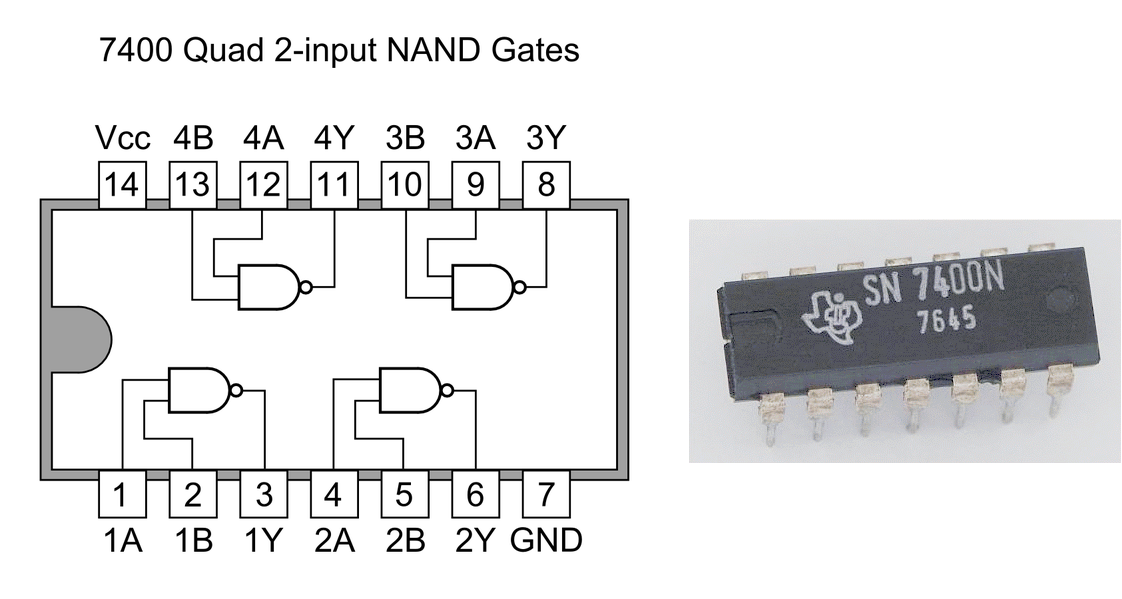
\includegraphics[width=13cm]{rap22rys3} 
\centering
\caption{Układ scalony.}
\end{figure}

W trakcie ćwiczeń badano właściwości układów: 7400, 7402 i 7474, które to składały się kolejno z: czterech bramek NAND, czterech bramek NOR i dwóch przerzutników typu D.
W końcowym etapem ćwiczeń było skonstruowanie stopera odliczającego od 0 do 99 wraz z funkcją stop oraz możliwością resetowania wartości.

\begin{center}
\textbf{\subsection*{UKŁAD DOŚWIADCZALNY}}
\end{center}

Układ doświadczalny składał się z makiety przedstawionej na Rysunku 4, generatora sygnałów, zasilacza napięcia stałego oraz szeregu układów scalonych: 7400, 7402, 7474 i 7490. 

\begin{figure}[h!]
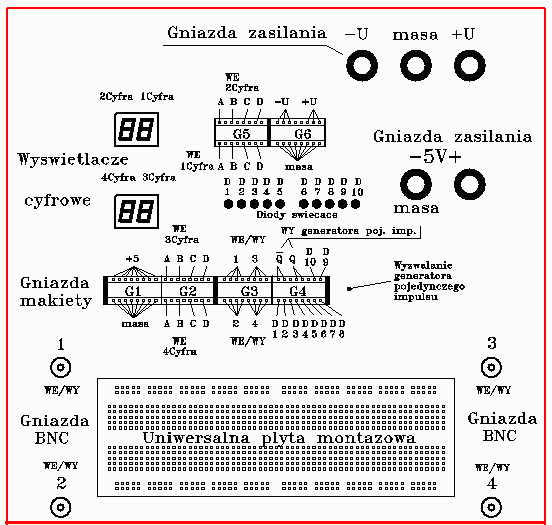
\includegraphics[width=11cm]{rap22rys4} 
\centering
\caption{Makieta \cite{r1}.}
\end{figure}

Do zacisków masy i 5V podłączono zasilacz. Generator sygnałów był podłączony do gniazda BNC nr 1, a układy scalone montowane były na uniwersalnej płytce montażowej.

\begin{center}
\textbf{\subsection*{BADANIE UKŁADÓW}}
\end{center}

W trakcie ćwiczeń skonstruowano z bramek NAND: sumę logiczną, iloczyn logiczny, implikację, zakaz i bramkę XOR. Korzystając z czterech przerzutników typu D skonstruowano licznik szesnastkowy, a łącząc go z bramkami NAND stworzono dekoder liczby 10, który zatrzymywał się po osiągnięciu liczby 9. Wszystkie te konstrukcje sprawdzano pod kątem zgodności z ich tabelami prawdy. Wykorzystano w tym celu diody świecące D1-D9, gdzie świecąca dioda symbolizowała "1", a nieświecąca "0". Po upewnieniu się ,ze wszystkie elementy spełniają swoje zadania, przystąpiono do projektowania i konstruowania stopera.


\begin{center}
\textbf{\subsection*{KONSTRUKCJA STOPERA}}
\end{center}

Schemat stopera przedstawiono na Rysunku 5. Układ scalony 7490 to układ składający się z licznika modulo 2 (wejście A i wyjście $Q_{A}$) oraz z licznika modulo 5 (reszta wejść i wyjść). Łącząc wyjście $Q_{A}$ z wejściem B otrzymujemy dekadę liczącą $-$ licznik modulo 10 zliczający od 0 do 9. Dodając kolejny tak samo przygotowany układ i łącząc wyjście $Q_{D}$ pierwszego licznika z wejściem A drugiego otrzymujemy licznik od 0 do 99. Za cyfrę jedności odpowiada pierwszy licznik, za cyfrę dziesiątek drugi, a stan na wyjściach Q jest reprezentacją binarną aktualnej wartości. 

\begin{figure}[h!]
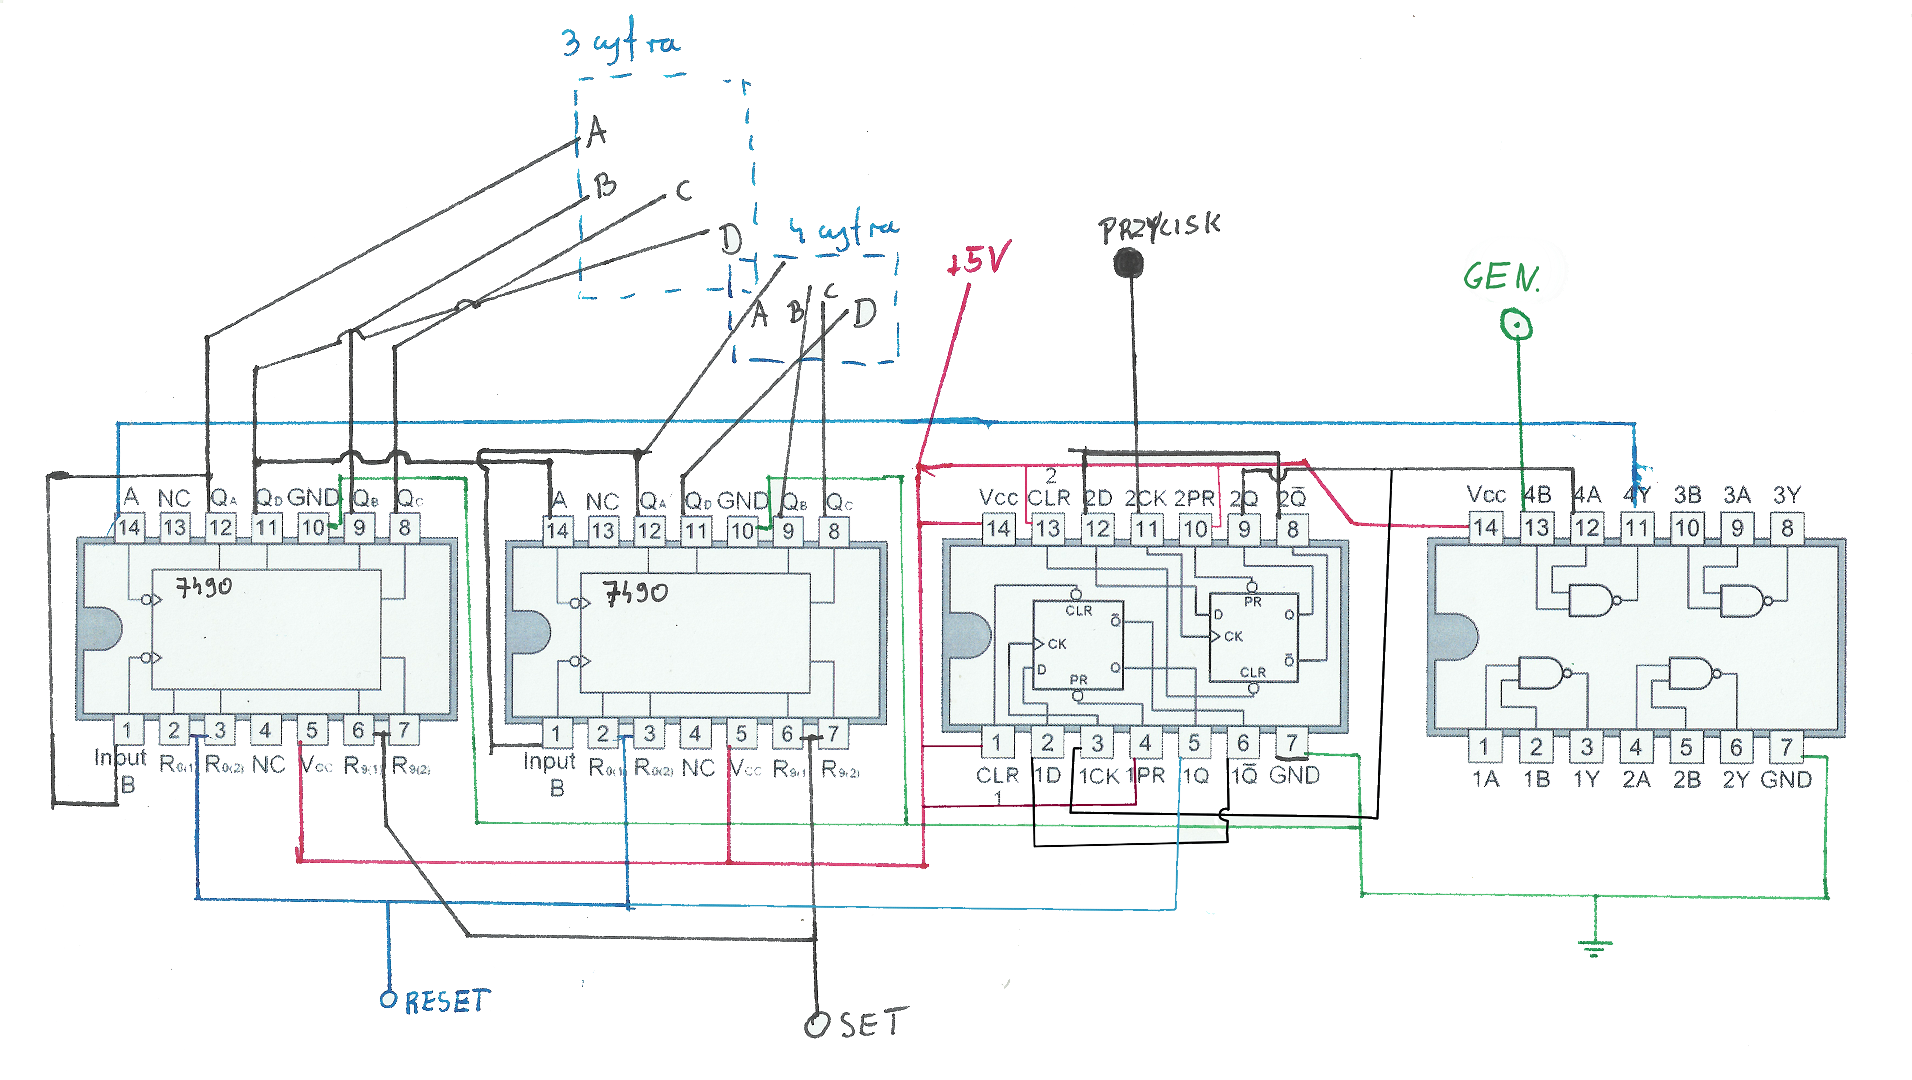
\includegraphics[width=13cm]{schemat3} 
\centering
\caption{Schemat stopera.}
\end{figure}

Wejście A pierwszego licznika jest połączone z wyjściem bramki NAND. Na wejściu tej bramki jest podłączony generator sygnału oraz przerzutnik typu D. Sam przerzutnik jest połączony w następujący sposób: wejście D przerzutnika jest połączone z wyjściem $\bar{Q}$ tego przerzutnika, a wejście zegara jest podłączone do przycisku na makiecie. W ten sposób, po każdym naciśnięciu przycisku przerzutnik zmienia swój stan, a w połączeniu z bramką NAND realizuje to funkcję start/stop. Dodatkowo wyjście Q tego przerzutnika jest połączone z zegarem innego, połączonego w analogiczny sposób. Wyjście Q drugiego układu połączone jest z wejściami reset obu liczników. W ten sposób po każdym cyklu start-stop uruchamiana jest opcja resetowania licznika. 

Wyjścia liczników podłączone są z wejściami Cyfry 3 dla jedności i Cyfry 4 dla dziesiątek. Do wejścia $i$ podłączone jest wyjście $Q_{i}$ licznika, gdzie $i$={A, B, C, D}. 

Stoper przetestowano dla sygnału wejściowego o częstości 10 Hz. Udało się osiągnąć poprawne zliczanie 0-99 oraz poprawne wykonywanie cyklu start-stop-reset. 

\begin{center}
\textbf{\subsection*{DYSKUSJA WYNIKÓW I WNIOSKI}}
\end{center}

Otrzymany stoper składał się z niewielu elementów i prostych połączeń jednocześnie realizując żądane funkcje. Można więc założyć, iż otrzymany układ był dobrze zoptymalizowany. Dodatkowo, ze względu na szybkie wykonanie zadania można stwierdzić, iż ćwiczenie zakończyło się pełnym sukcesem.

\begin{center}
\begin{thebibliography}{9}

\bibitem{r1}
 Praca zbiorowa,
 \emph{Instrukcja do ćwiczenia "Cyfrowe układy scalone"},
 FUW, Warszawa, 2016.
 
 
 
 \end{thebibliography}

\end{center}


\end{document}